\chapter{Three Ways to Work}
\label{ch:modes}

\algolang\ can be used in three ways, from the simplest to the most powerful. All three use the same compiler and runtime, so a program written one way runs unchanged in the others.

\begin{center}
\small
\begin{tabularx}{\linewidth}{@{}L{2.6cm}L{5.0cm}Y@{}}
\toprule
\thead{Way} & \thead{Start it with} & \thead{Best for}\\
\goldrule
\textbf{Simple} & \code{algo} (menu), \code{algo shell}, \code{algo run} & Quick runs, scripts, lab sessions\\
\textbf{Graphical} & \code{algo studio} & Writing, running and seeing programs in a browser\\
\textbf{Agentic} & \code{algo ask "…"}, \code{algo wizard} & Letting AI write the program, or answering questions to build one\\
\bottomrule
\end{tabularx}
\end{center}

\section{Simple: the menu}

Type \code{algo} on its own and a numbered menu offers every option. No commands need to be remembered.

\begin{terminal}
$ algo

  AlgoLang 0.2.0 — every unit of work is an agent

   SIMPLE (command line)
     1  Create a new program           4  Interactive shell
     2  Run a program                  5  Environment check
     3  Check a program for errors
   GRAPHICAL
     6  AlgoLang Studio (opens in your browser)
     7  Jupyter notebook
   AGENTIC
     8  Ask AI to write a program from your description
     9  Wizard: build a program by answering questions (no AI)

     0  Exit

  Choose 0-9:
\end{terminal}

\section{Simple: the interactive shell}

\code{algo shell} lets you type \algolang\ one declaration at a time, like the Python prompt. A block continues until its braces balance. Each declaration is checked as soon as it is complete; one with errors is rejected and explained, and the session is left unchanged. Calling an agent directly runs it at once.

\begin{terminal}
$ algo shell
AlgoLang 0.2.0 shell — every unit of work is an agent
algo> model fast = "claude-haiku-5-5"
✓ model fast
algo> agent Explainer(topic: text) -> text {
...>     goal "Explain {topic} simply"
...>     model fast
...> }
✓ Explainer
algo> agent Bad(x: text) -> text {
...>     goal "use {y}"
...> }
✗ not added — 1 error(s):
  E109 line 1: agent Bad: goal mentions {y} but there is no parameter 'y'
algo> // … QuizMaker and flow main are added the same way …
algo> Explainer("graph neural networks")
▶ flow main  run=f6150c29  backend=mock
  → Explainer          conf=0.64  «Explainer #8884» Explain graph neural networks simply
algo> :graph
  ◇ topic                      flow input
  ■ Explainer                  → lesson                  ← topic
  ■ QuizMaker                  → quiz                    ← Explainer
  ◎ emit                       flow output               ← Explainer, QuizMaker
algo> :save lesson.algo
✓ saved lesson.algo
\end{terminal}

\begin{center}
\small
\begin{tabularx}{\linewidth}{@{}L{4.4cm}Y@{}}
\toprule
\thead{Shell command} & \thead{Effect}\\
\goldrule
\code{:run topic=AI} & Run \code{flow main}; missing inputs are asked for\\
\code{:check}, \code{:graph}, \code{:python} & Check, show agent connections, show generated Python\\
\code{:list}, \code{:show} & List definitions; print the whole program\\
\code{:save f.algo}, \code{:load f.algo} & Save or load a program\\
\code{:live on|off} & Switch between real Claude models and the offline mock\\
\code{:reset}, \code{:help}, \code{:quit} & Start again; help; leave\\
\bottomrule
\end{tabularx}
\end{center}

\section{Graphical: AlgoLang Studio}

\code{algo studio} starts a small server on your own computer and opens \emph{AlgoLang Studio} in your web browser (Figure~\ref{fig:studio}). Nothing leaves your machine unless you switch on live mode.

\begin{figure}[ht]
\centering
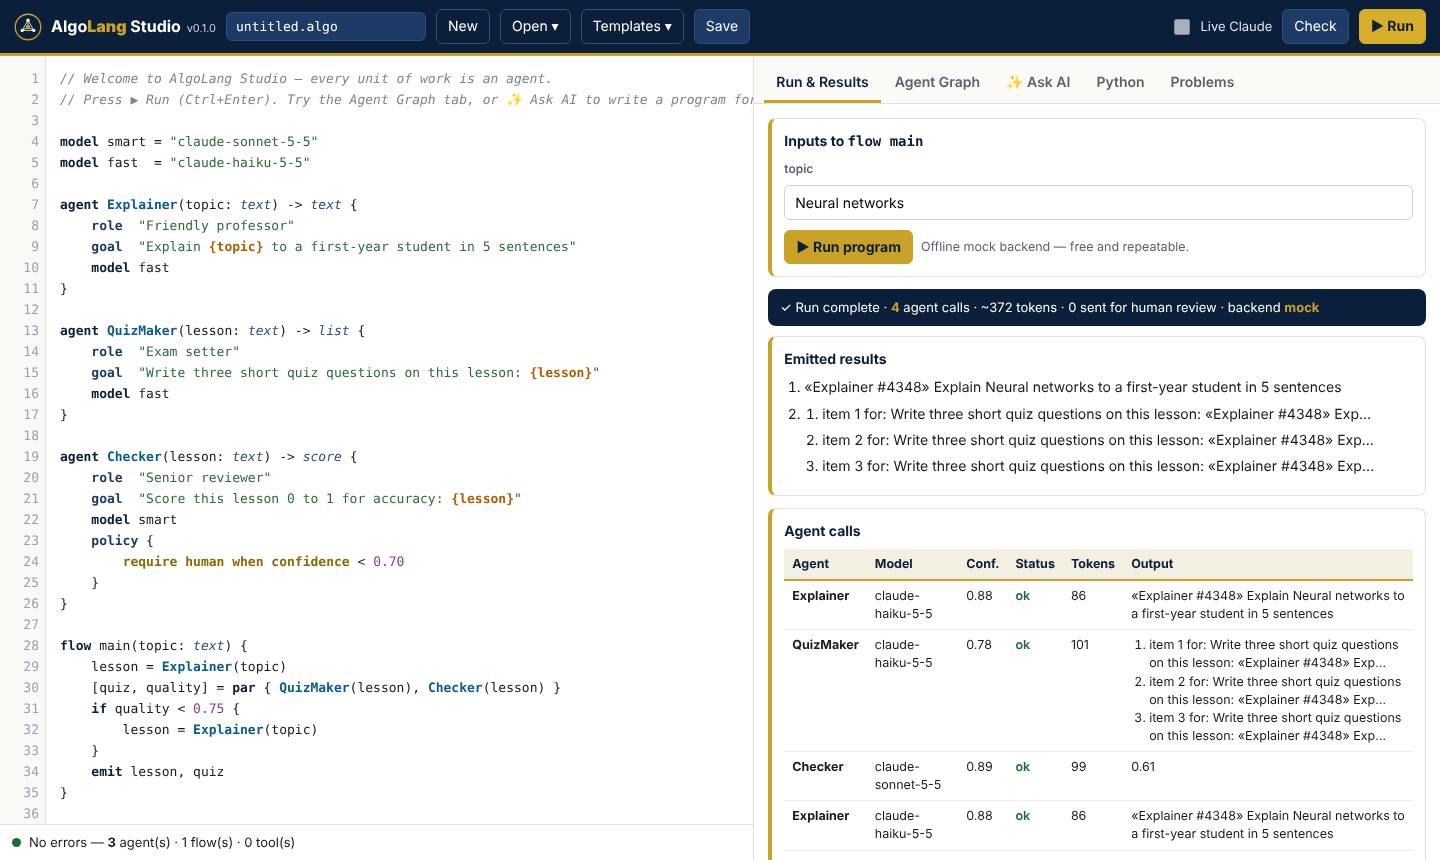
\includegraphics[width=\linewidth]{images/studio-run.png}
\caption{AlgoLang Studio after a run: the editor with highlighting and live error checking (left), and the inputs, emitted results and agent-call table (right).}
\label{fig:studio}
\end{figure}

\begin{center}
\small
\begin{tabularx}{\linewidth}{@{}L{3.2cm}Y@{}}
\toprule
\thead{Area} & \thead{What it does}\\
\goldrule
Editor & Syntax highlighting, line numbers, automatic indentation; errors marked in red in the margin as you type\\
\texttt{▶} Run (Ctrl+Enter) & Fills in a form for \code{flow main}'s inputs, runs, and shows results, confidences, human-review flags and the audit-log path\\
Agent Graph & Draws the flow top to bottom (Figure~\ref{fig:studiograph})\\
Ask AI & Describe a program in plain English; AI writes it (Section~\ref{sec:ask})\\
Templates & Start from any of six design patterns, no AI needed\\
Python & The code the compiler generates\\
Problems & Every compile error; click one to jump to its line\\
Open / Save & Your programs in the workspace folder, and the examples\\
Live Claude & Switches from the offline mock to real models (needs an API key)\\
\bottomrule
\end{tabularx}
\end{center}

\begin{figure}[ht]
\centering
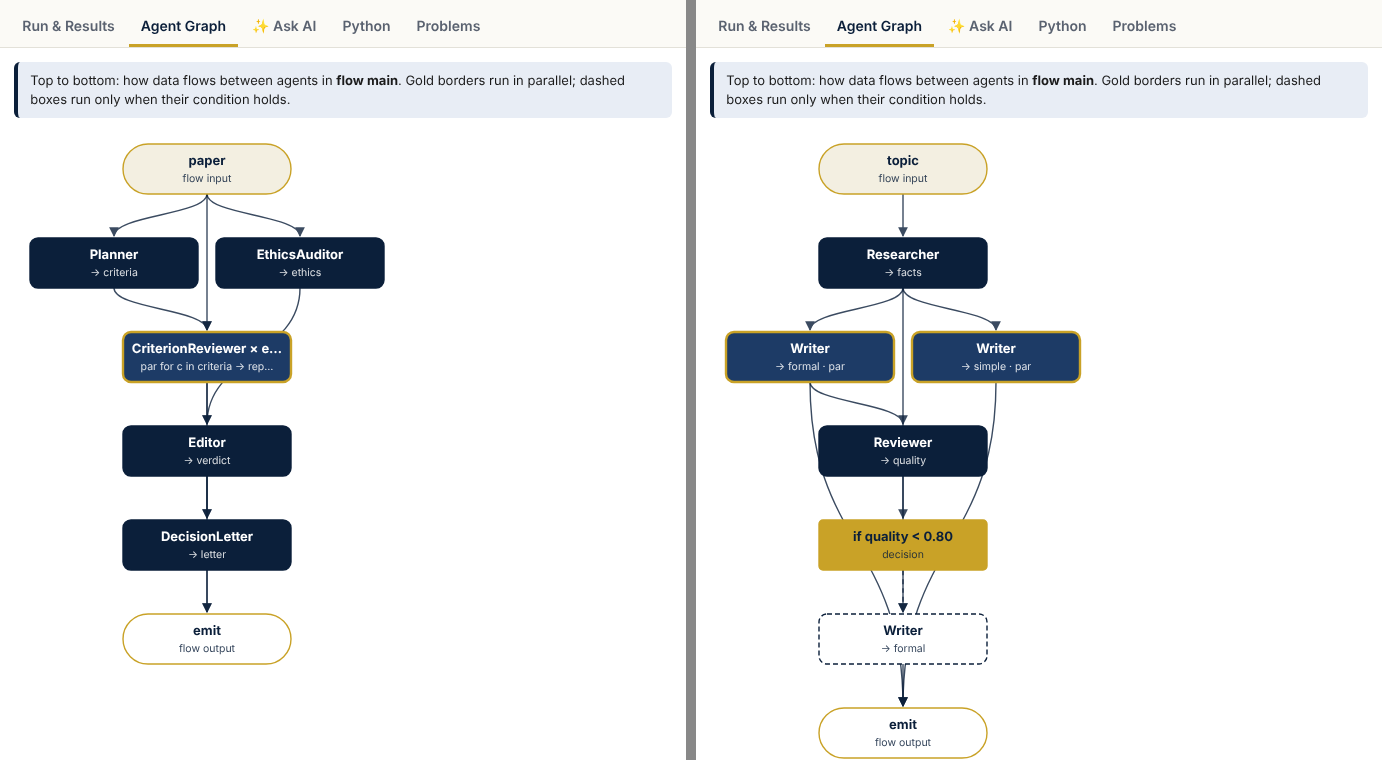
\includegraphics[width=0.92\linewidth]{images/studio-graphs.png}
\caption{Agent Graph for the paper-review program (left) and the research-brief program (right). Gold borders mark agents that run in parallel; the dashed box runs only when its condition holds.}
\label{fig:studiograph}
\end{figure}

\begin{note}
Studio listens only on \code{127.0.0.1} and refuses requests from other web sites, so other pages open in your browser cannot use it. Use \code{algo studio --port 9000} to choose a port, or \code{--no-browser} to start it without opening a window.
\end{note}

\section{Agentic: AI writes the program}
\label{sec:ask}

\code{algo ask} turns a description into a working \algolang\ program:

\begin{terminal}
$ algo ask "build a team that reviews a research paper and drafts a decision letter"
\end{terminal}

Behind the command is a small agentic loop, shown in Figure~\ref{fig:askloop}:

\begin{enumerate}
  \item A model receives your request together with a concise guide to \algolang's rules and an example.
  \item Its program is compiled by the real \algolang\ compiler.
  \item If there are errors, the exact compiler messages are sent back to the model to fix.
  \item This repeats up to three times. A program is accepted only when it compiles with \textbf{zero errors}; then it is saved and printed, and \code{--run} runs it immediately.
\end{enumerate}

\begin{figure}[ht]
\centering
\begin{tikzpicture}[
  st/.style={fill=navy,text=white,rounded corners=3pt,font=\sffamily\scriptsize,minimum width=24mm,minimum height=11mm,align=center},
  ok/.style={st,fill=strgreen},
  ch/.style={st,fill=gold,text=navy,font=\sffamily\scriptsize\bfseries},
  ar/.style={-{Stealth[length=2mm]},navy,line width=0.7pt}]
  \node[st] (r) {your\\request};
  \node[st,right=6mm of r] (m) {model writes\\AlgoLang};
  \node[ch,right=6mm of m] (c) {compiler\\checks};
  \node[ok,right=16mm of c] (s) {save + run\\(0 errors)};
  \draw[ar] (r) -- (m); \draw[ar] (m) -- (c); \draw[ar] (c) -- node[above,font=\sffamily\tiny]{no errors} (s);
  \draw[ar,cautionred] (c.south) -- ++(0,-6mm) -| node[pos=0.25,below,font=\sffamily\tiny,text=cautionred]{errors sent back (max 3 attempts)} (m.south);
\end{tikzpicture}
\caption{The write–compile–repair loop behind \code{algo ask} and Studio's Ask AI.}
\label{fig:askloop}
\end{figure}

The output shows each attempt. Here a first draft used an undefined placeholder and called a function; the compiler's messages were returned to the model, and the second attempt compiled:

\begin{terminal}
→ attempt 1: asking claude-sonnet-5-5 to write the program…
✗ attempt 1: 2 compile error(s) — sending them back to be fixed
    line 2: E109 agent Reviewer: goal mentions {manuscript} but there is no parameter 'manuscript'
    line 7: E101 'summarise' is not an agent — in AlgoLang every unit of work is an agent …
→ attempt 2: asking claude-sonnet-5-5 to write the program…
✓ attempt 2: compiles with no errors
\end{terminal}

\begin{ethics}[Generated programs still need review]
The compiler guarantees that a generated program is \emph{well-formed}: names, types, tools and policies are consistent. It cannot guarantee that the program does what you intended, or that its goals, thresholds and forbidden attributes are the right ones. Read every generated program before you run it live, exactly as you would review code written by a colleague.
\end{ethics}

\code{algo ask} needs \code{ANTHROPIC\_API\_KEY} and the \code{anthropic} package (Section~\ref{sec:live-setup}). The model can be changed with the environment variable \code{ALGO\_ASK\_MODEL}.

\section{Agentic without AI: the wizard}

\code{algo wizard} builds a program by asking six short questions. Pressing Enter accepts each default, so a complete program takes seconds:

\begin{terminal}
$ algo wizard
1. What should your AI system do [answer student questions about AI]: help students prepare for viva exams
2. Choose a design pattern:
   1. Pipeline — research, write, then edit, one after another
   2. Fan-out / fan-in — plan the parts, work on each in parallel, combine
   3. Committee — three experts answer in parallel, a judge decides
   4. Critic & revise — draft, score, redraft if the score is low
   5. Router — classify the input and send it to the right specialist
   6. Guardrail — safety check first, then do the work
   Pattern number [2]: 3
3. Name of the input (one word) [request]: question
4. Send low-confidence decisions to a human? (y/n) [y]:
   Confidence threshold (0-1) [0.75]: 0.8
5. Forbid protected attributes in decisions? (y/n) [y]:
   Which ones [gender, caste, religion, nationality]:
6. Token budget per agent [4000]: 3000
✓ wrote help_students_prepare_for_viva.algo (committee pattern) — it compiles with no errors.
\end{terminal}

The wizard's programs are built from the patterns of Chapter~\ref{ch:patterns}, with human review, budgets and protected-attribute rules placed on the agent that makes the final decision. They always compile, and they are a good starting point to edit by hand or in Studio.
